\documentclass[tikz,border=6pt]{standalone}
\usepackage{amsmath}
\usetikzlibrary{arrows.meta,positioning,calc,fit}
\begin{document}
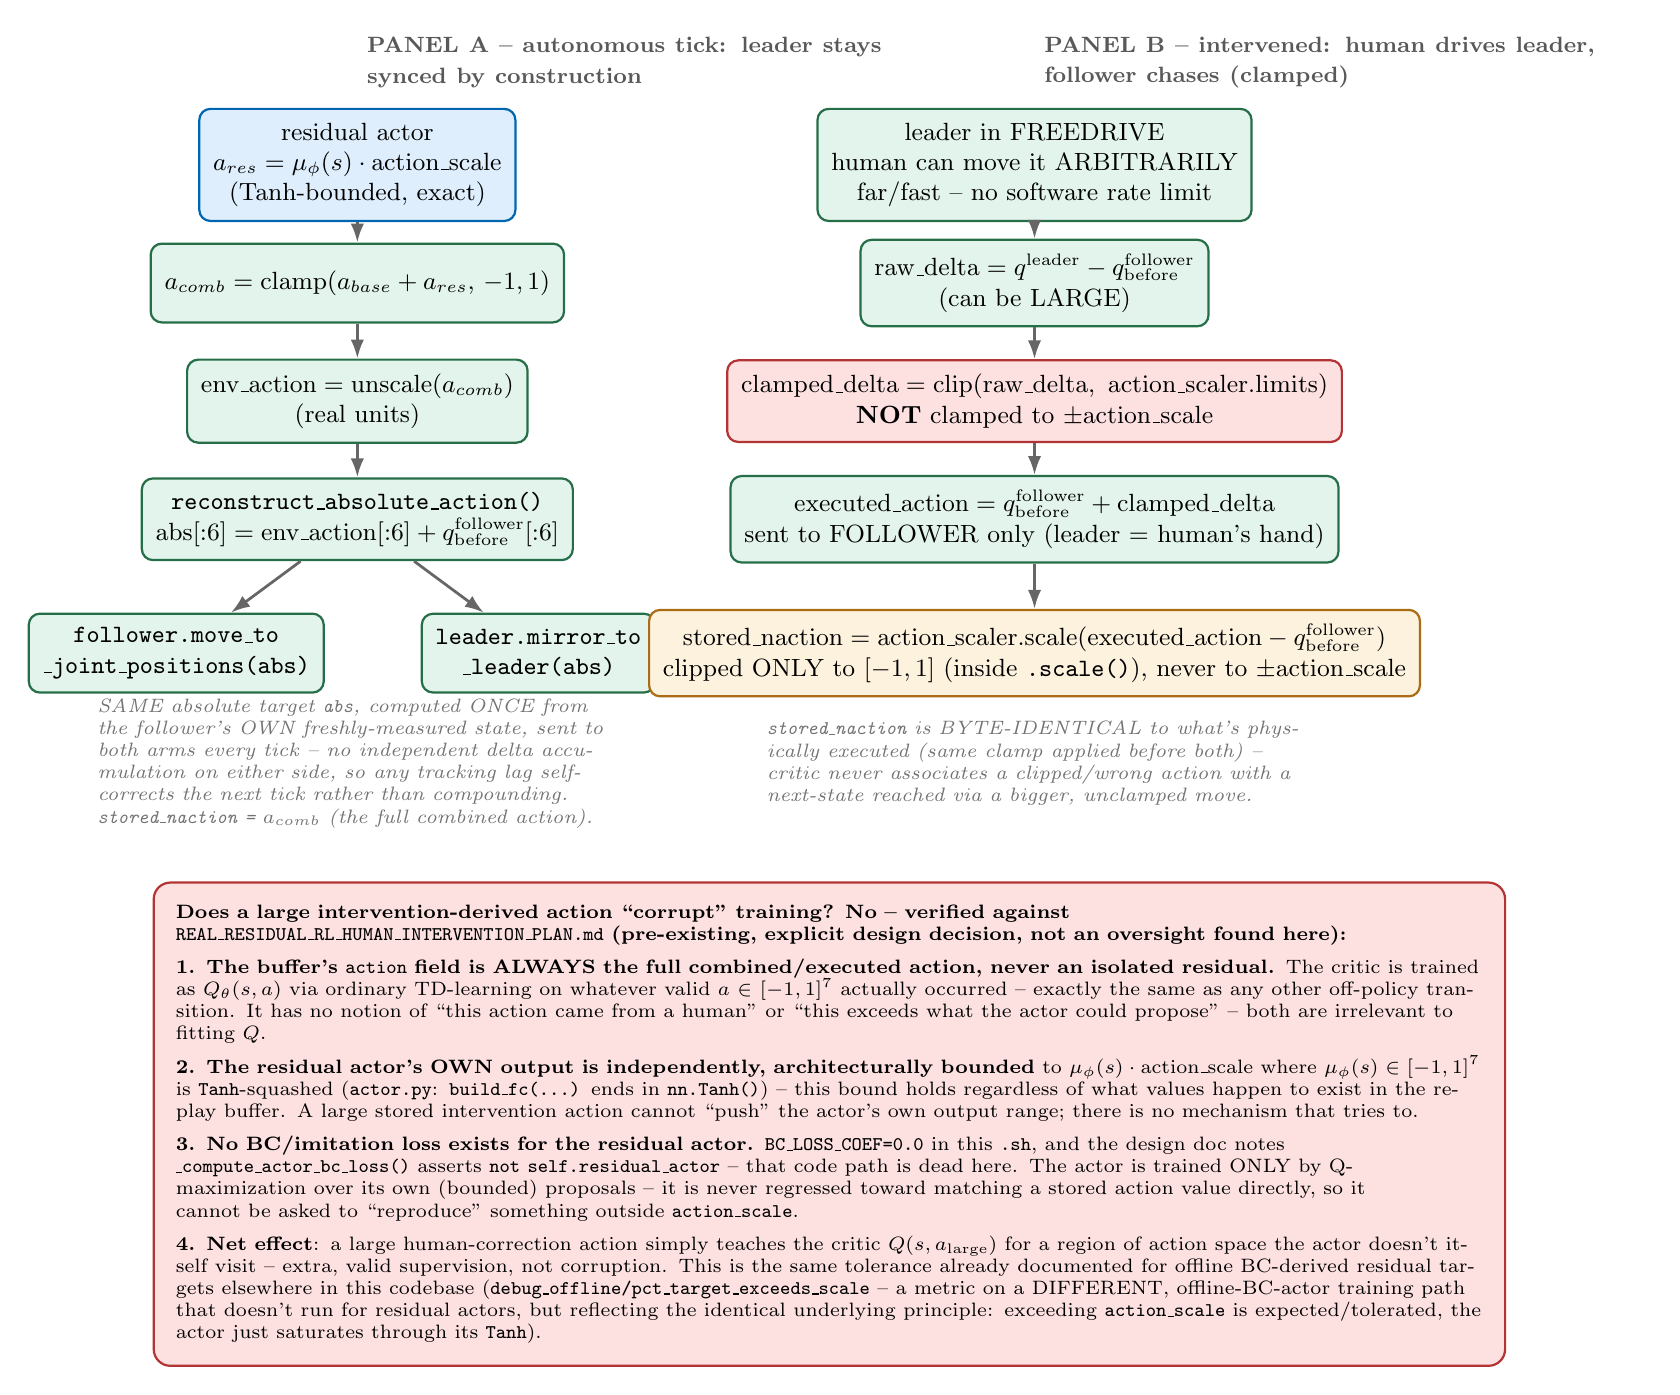
\begin{tikzpicture}[
    >={Latex[length=2.4mm,width=1.7mm]}, font=\small,
    box/.style={draw,thick,rounded corners=4pt,align=center,minimum height=1.0cm,inner sep=5pt,fill=white},
    actor/.style={box,draw=actline,fill=actfill},
    env/.style={box,draw=envline,fill=envfill},
    buf/.style={box,draw=bufline,fill=buffill},
    warn/.style={box,draw=doneline,fill=donefill},
    flow/.style={->,line width=1.0pt,draw=black!60},
    hdr/.style={font=\small\bfseries,text=black!65},
    lbl/.style={font=\scriptsize,align=left,text=black!65},
    note/.style={font=\scriptsize\itshape,align=left,text=black!55},
]
\definecolor{actline}{RGB}{0,102,178}   \definecolor{actfill}{RGB}{222,238,252}
\definecolor{envline}{RGB}{38,110,72}   \definecolor{envfill}{RGB}{226,244,235}
\definecolor{bufline}{RGB}{170,108,20}  \definecolor{buffill}{RGB}{252,242,222}
\definecolor{doneline}{RGB}{178,52,52}  \definecolor{donefill}{RGB}{253,225,225}

% ================= PANEL A: autonomous (not intervened) - the sync mechanism =================
\node[hdr,text width=7.6cm,align=left] at (0,9.0) [anchor=west] {\footnotesize PANEL A -- autonomous tick: leader stays synced by construction};

\node[actor] (a1) at (0,7.7) {residual actor\\$a_{res}=\mu_\phi(s)\cdot\text{action\_scale}$\\(Tanh-bounded, exact)};
\node[env] (a2) at (0,6.2) {$a_{comb}=\mathrm{clamp}(a_{base}+a_{res},\,-1,1)$};
\node[env] (a3) at (0,4.7) {$\text{env\_action}=\text{unscale}(a_{comb})$\\(real units)};
\node[env] (a4) at (0,3.2) {\texttt{reconstruct\_absolute\_action()}\\$\text{abs}[{:}6]=\text{env\_action}[{:}6]+q^{\text{follower}}_{\text{before}}[{:}6]$};
\node[env] (a5f) at (-2.3,1.5) {\texttt{follower.move\_to}\\\texttt{\_joint\_positions(abs)}};
\node[env] (a5l) at (2.3,1.5) {\texttt{leader.mirror\_to}\\\texttt{\_leader(abs)}};

\draw[flow] (a1) -- (a2);
\draw[flow] (a2) -- (a3);
\draw[flow] (a3) -- (a4);
\draw[flow] (a4) -- (a5f);
\draw[flow] (a4) -- (a5l);

\node[note,text width=6.6cm] at (0,0.1) {SAME absolute target \texttt{abs}, computed ONCE from the follower's OWN freshly-measured state, sent to both arms every tick -- no independent delta accumulation on either side, so any tracking lag self-corrects the next tick rather than compounding. \texttt{stored\_naction = }$a_{comb}$ (the full combined action).};

% ================= PANEL B: intervened - the clip-and-store mechanism =================
\node[hdr,text width=7.6cm,align=left] at (8.6,9.0) [anchor=west] {\footnotesize PANEL B -- intervened: human drives leader, follower chases (clamped)};

\node[env] (b1) at (8.6,7.7) {leader in FREEDRIVE\\human can move it ARBITRARILY\\far/fast -- no software rate limit};
\node[env] (b2) at (8.6,6.2) {$\text{raw\_delta}=q^{\text{leader}}-q^{\text{follower}}_{\text{before}}$\\(can be LARGE)};
\node[warn] (b3) at (8.6,4.7) {$\text{clamped\_delta}=\mathrm{clip}(\text{raw\_delta},\ \text{action\_scaler.limits})$\\\textbf{NOT} clamped to $\pm\text{action\_scale}$};
\node[env] (b4) at (8.6,3.2) {$\text{executed\_action}=q^{\text{follower}}_{\text{before}}+\text{clamped\_delta}$\\sent to FOLLOWER only (leader = human's hand)};
\node[buf] (b5) at (8.6,1.5) {$\text{stored\_naction}=\text{action\_scaler.scale}(\text{executed\_action}-q^{\text{follower}}_{\text{before}})$\\clipped ONLY to $[-1,1]$ (inside \texttt{.scale()}), never to $\pm$action\_scale};

\draw[flow] (b1) -- (b2);
\draw[flow] (b2) -- (b3);
\draw[flow] (b3) -- (b4);
\draw[flow] (b4) -- (b5);

\node[note,text width=6.8cm] at (8.6,0.1) {\texttt{stored\_naction} is BYTE-IDENTICAL to what's physically executed (same clamp applied before both) -- critic never associates a clipped/wrong action with a next-state reached via a bigger, unclamped move.};

% ================= CONCLUSION BOX =================
\node[draw=doneline,thick,rounded corners=6pt,fill=donefill,align=left,font=\scriptsize,
      inner sep=8pt,text width=16.6cm,anchor=north west] at (-2.6,-1.4) {
  \textbf{Does a large intervention-derived action ``corrupt'' training? No -- verified against \texttt{REAL\_RESIDUAL\_RL\_HUMAN\_INTERVENTION\_PLAN.md} (pre-existing, explicit design decision, not an oversight found here):}\\[4pt]
  \textbf{1. The buffer's \texttt{action} field is ALWAYS the full combined/executed action, never an isolated residual.} The critic is trained as $Q_\theta(s,a)$ via ordinary TD-learning on whatever valid $a\in[-1,1]^7$ actually occurred -- exactly the same as any other off-policy transition. It has no notion of ``this action came from a human'' or ``this exceeds what the actor could propose'' -- both are irrelevant to fitting $Q$.\\[4pt]
  \textbf{2. The residual actor's OWN output is independently, architecturally bounded} to $\mu_\phi(s)\cdot\text{action\_scale}$ where $\mu_\phi(s)\in[-1,1]^7$ is \texttt{Tanh}-squashed (\texttt{actor.py}: \texttt{build\_fc(...)} ends in \texttt{nn.Tanh()}) -- this bound holds regardless of what values happen to exist in the replay buffer. A large stored intervention action cannot ``push'' the actor's own output range; there is no mechanism that tries to.\\[4pt]
  \textbf{3. No BC/imitation loss exists for the residual actor.} \texttt{BC\_LOSS\_COEF=0.0} in this \texttt{.sh}, and the design doc notes \texttt{\_compute\_actor\_bc\_loss()} asserts \texttt{not self.residual\_actor} -- that code path is dead here. The actor is trained ONLY by Q-maximization over its own (bounded) proposals -- it is never regressed toward matching a stored action value directly, so it cannot be asked to ``reproduce'' something outside \texttt{action\_scale}.\\[4pt]
  \textbf{4. Net effect}: a large human-correction action simply teaches the critic $Q(s, a_{\text{large}})$ for a region of action space the actor doesn't itself visit -- extra, valid supervision, not corruption. This is the same tolerance already documented for offline BC-derived residual targets elsewhere in this codebase (\texttt{debug\_offline/pct\_target\_exceeds\_scale} -- a metric on a DIFFERENT, offline-BC-actor training path that doesn't run for residual actors, but reflecting the identical underlying principle: exceeding \texttt{action\_scale} is expected/tolerated, the actor just saturates through its \texttt{Tanh}).
};

\end{tikzpicture}
\end{document}
